\def\pgfsysdriver{pgfsys-dvisvgm.def}
% flashcards-title: Matched plant groups differing in one added material
% flashcards-desc: Group A and Group B each show three plant symbols in matching pots under the same light. Equal-volume containers are labeled plain water for A and water plus added material for B.
\documentclass[tikz,border=6pt]{standalone}
\usetikzlibrary{arrows.meta,calc,fit,positioning,shapes.geometric}

\definecolor{fcink}{HTML}{17212B}
\definecolor{fcblue}{HTML}{1D5D8C}
\definecolor{fcgreen}{HTML}{2D6A4F}
\definecolor{fcorange}{HTML}{A44A1F}
\definecolor{fcpale}{HTML}{F4F7F9}
\definecolor{fcsoil}{HTML}{8B5E3C}

\tikzset{
  fc text/.style={font=\sffamily, text=fcink},
  fc panel/.style={draw=fcink, line width=0.9pt, rounded corners=5pt, fill=fcpale},
  fc node/.style={draw=fcink, line width=0.9pt, rounded corners=4pt, fill=white,
    minimum width=24mm, minimum height=10mm, align=center, font=\sffamily},
  fc arrow/.style={-{Stealth[length=3.2mm,width=2.4mm]}, line width=1.2pt,
    draw=fcblue, line cap=butt},
  fc boundary/.style={draw=fcorange, line width=1.4pt, dash pattern=on 5pt off 3pt,
    rounded corners=7pt},
  fc label/.style={font=\sffamily\bfseries, text=fcink},
  fc note/.style={font=\sffamily\small, text=fcink, align=center}
}

\begin{document}
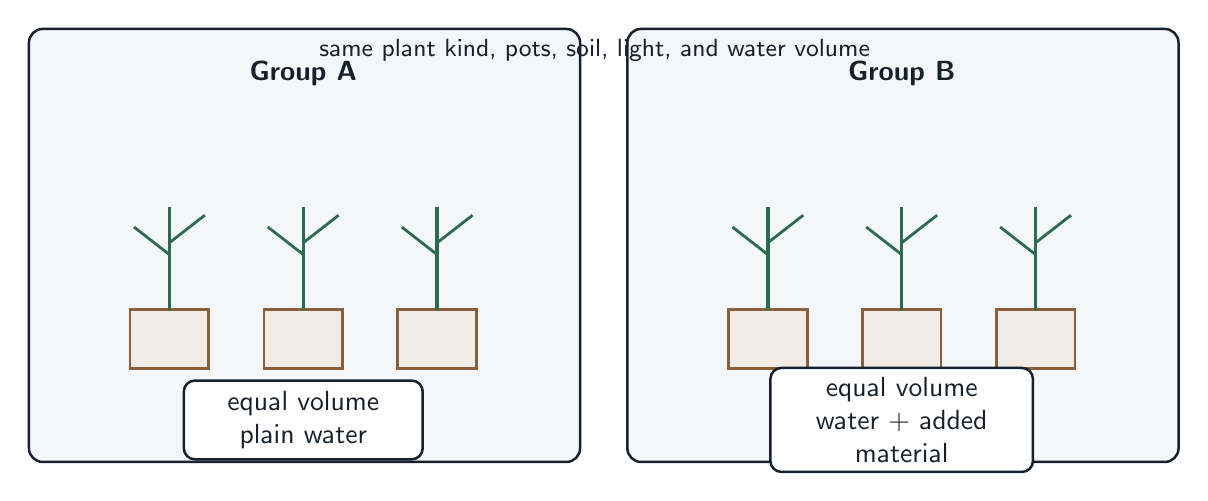
\begin{tikzpicture}[fc text, x=1cm, y=1cm]
  \node[fc panel, minimum width=70mm, minimum height=55mm, anchor=south west] at (0,0) {};
  \node[fc panel, minimum width=70mm, minimum height=55mm, anchor=south west] at (7.6,0) {};
  \node[fc label] at (3.5,4.95) {Group A};
  \node[fc label] at (11.1,4.95) {Group B};
  \foreach \o in {0,7.6} {
    \foreach \x in {1.3,3.0,4.7} {
      \draw[draw=fcsoil, fill=fcsoil!12, line width=1pt] (\o+\x,1.2) rectangle +(1.0,.75);
      \draw[draw=fcgreen, line width=1.2pt] (\o+\x+.5,1.95)--+(0,1.3);
      \draw[draw=fcgreen, line width=1pt] (\o+\x+.5,2.65)--+(-.45,.35) (\o+\x+.5,2.8)--+(.45,.35);
    }
  }
  \node[fc node, text width=28mm] at (3.5,.55) {equal volume\\plain water};
  \node[fc node, text width=31mm] at (11.1,.55) {equal volume\\water + added material};
  \node[fc note] at (7.2,5.25) {same plant kind, pots, soil, light, and water volume};
\end{tikzpicture}
\end{document}
